
\section{Background}
% TODO :Description of the scientific area/problem that gave rise to the dataset. Place the dataset in context, providing sufficient references for the reader to understand the importance and significance of the data. What kind of analyses have been done in the literature?

The chosen dataset is daily updated and contains reported crimes in the City of Chicago from the year 2001 to present time except for the last seven days. The data is originally generated by the Chicago Police Department’s CLEAR (Citizen Law Enforcement Analysis and Reporting) system, which is a system for government agencies in the Chicago area to share information about crime and criminal records between each other \cite{CLEARpolice}. CLEAR is not available to the public, but parts of it is published in the Chicago Open Data Portal, provided by the city of Chicago, which was the source for the dataset used in this project. 
\bigbreak
The specific dataset used is called “Crimes - 2001 to present” and is presented under the “Public Safety” category of the Chicago Open Data Portal and contains approximately 6,6 million reported crimes during the time period. The data is showing details such as crime type, date, location, arrest, etc. An exact address of the crime location is not provided in this public dataset for privacy reasons, but the street block address is provided for approximate geographical location \cite{cityOfChicago}. 
\bigbreak
The Chicago Open Data Portal has done some analyses on the data already which is provided as graphs in the portal for easy overview. These include graphs showing the aggregated number of crimes per month, number of crimes by primary type (as seen in figure \ref{fig:exampleGraph}), crime arrest percentage, ratio between domestic or non domestic crimes and maps showing crime rate in different police districts and zip codes are presented. 

\begin{figure}[H]
    \centering
    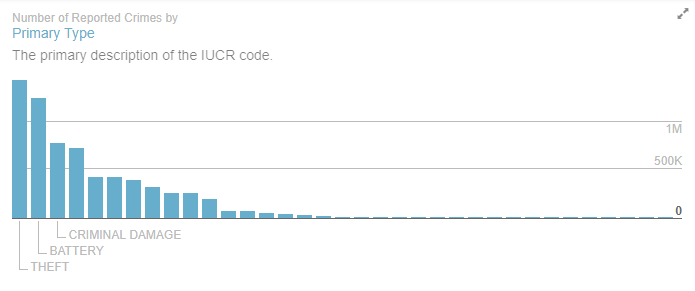
\includegraphics[width=.95\linewidth]{figures/existingPrimaryType.PNG}
    \caption{Graph from Chicago Open Data Portal showing crimes sorted by primary crime type \cite{cityOfChicago}.}
    \label{fig:exampleGraph}
\end{figure}

\pagebreak